\begin{NuevaPagina}{64}{94}{show1}
	%------------------------------CABECERA----------------------------
	\CabeceraDePoster{\MATERIA} 
	\begin{NuevoParrafo}{0}{76}[18][6]
		\begin{Marco}[\LineaSupC][\LineaInfC][\LineaIzqC][\LineaDerC][CBlanco]
			\autores{Sergio Cardenas - Cod:20192020126}{Stivel Pinilla - Cod:20191020024}{Juan Mancera - Cod:20171020047}
		\end{Marco}
	\end{NuevoParrafo} 
	%-------------------------------DIVISION--------------------------
	\CiudadFechaVolumen
	%----------------------------MISION/VISION------------------------
	\CabeceraDeSubSeccionConAnchoN{9}{0}{14}{80}{FARMA-WEB}{CTDiario}{CCDiario}
	\begin{NuevoParrafo}{11}{0}[46][6]
		\begin{Marco}[\LineaSupC][\LineaInfC][\LineaIzqC][\LineaDerC][CBlanco]
			\begin{MisionVision}[Misión]
				{Desarrollar soluciones tecnológicas innovadoras de monitoreo y análisis de la calidad del aire que integren ciencia de datos y usabilidad, con el fin de proporcionar información clara, confiable y accesible a la ciudadanía de Bogotá, a las entidades ambientales y a la comunidad científica. Nuestro compromiso es impulsar decisiones más conscientes y políticas públicas efectivas que promuevan un ambiente más saludable y sostenible.}
			\end{MisionVision}			
		\end{Marco}
	\end{NuevoParrafo}
	%\CabeceraDeSubSeccionConAnchoN{4}{0}{7}{39}{FARMA-WEB}{CTDiario}{CCDiario}
	\begin{NuevoParrafo}{17}{0}[46][6]
		\begin{Marco}[\LineaSupC][\LineaInfC][\LineaIzqC][\LineaDerC][CBlanco]
			\begin{MisionVision}[Visión]
				{Ser en el año 2030 la empresa líder en Colombia en el desarrollo de software de calidad del aire, reconocida por su impacto en la toma de decisiones ambientales, su aporte a la investigación científica y su capacidad de empoderar a la ciudadanía con herramientas digitales que contribuyan a mejorar la salud pública y la sostenibilidad urbana.}
			\end{MisionVision}
		\end{Marco}
	\end{NuevoParrafo}
		\begin{NuevoParrafo}{11}{48}[46][12]
		\begin{Marco}[\LineaSupC][\LineaInfC][\LineaIzqC][\LineaDerC][CBlanco]
			\begin{Objetivos}[Objetivos]
				{	{\large General:}\vspace{5pt}\\
					{\linespread{.8}\selectfont Desarrollar un software de monitoreo y análisis de la calidad del aire en Bogotá que integre datos ambientales de distintas fuentes oficiales, brinde visualizaciones intuitivas y facilite la toma de decisiones informadas por parte de la ciudadanía, las entidades gubernamentales y la comunidad científica.}\\[0.3cm]
					{\large Específicos:}
					{\begin{itemize}
							\setlength{\itemsep}{-0.5pt}
							\setlength{\parskip}{0pt}
							\setlength{\parsep}{0pt}
							\item Diseñar una plataforma digital con interfaces accesibles y usables que permitan a los usuarios finales consultar información clara y confiable sobre la calidad del aire en tiempo real.
							\item Implementar modelos de análisis de datos e indicadores ambientales que apoyen la formulación de políticas públicas, investigaciones científicas y programas de educación ambiental en Bogotá.
					\end{itemize}}
				}
			\end{Objetivos}
		\end{Marco}
	\end{NuevoParrafo}
	
	%----------------CAPA DE MOTIVACION------------------------------------------	
	
	\CabeceraDeSubSeccionConAnchoN{23}{0}{14}{80}{MOTIVACION}{CTDiario}{CCDiario}
	\begin{NuevoParrafo}{26}{41}[26][15]
		\begin{Marco}[\LineaSupC][\LineaInfC][\LineaIzqC][\LineaDerC][CBlanco]
		\subseccionC{\PVSta}%{CTSeccionPrimeraPlana}{CCSeccionPrimeraPlana} 
		\centering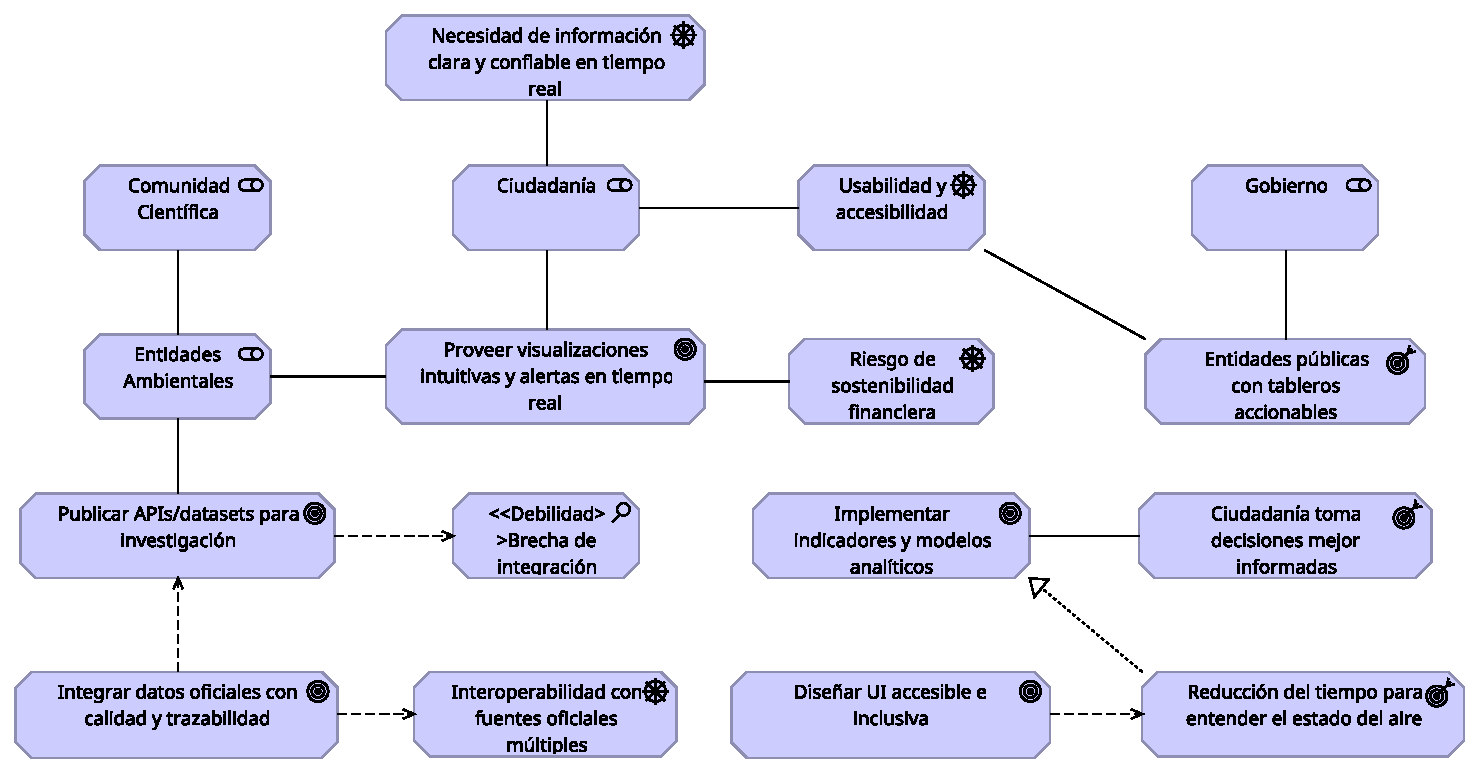
\includegraphics[scale=0.50]{\RCR/motivacion/Stakeholders.pdf}
		\end{Marco}
	\end{NuevoParrafo}

	\begin{NuevoParrafo}{26}{68}[26][15]
		\begin{Marco}[\LineaSupC][\LineaInfC][\LineaIzqC][\LineaDerC][CBlanco]
			\subseccionC{\PVPri}%{CTSeccionPrimeraPlana}{CCSeccionPrimeraPlana} 
			\centering\includegraphics[scale=0.55]{\RCR/motivacion/Principios.pdf}
		\end{Marco}
	\end{NuevoParrafo}
	
	\begin{NuevoParrafo}{47}{0}[20][15]
		\begin{Marco}[\LineaSupC][\LineaInfC][\LineaIzqC][\LineaDerC][CBlanco]
			\subseccionC{\PVROb}%{CTSeccionPrimeraPlana}{CCSeccionPrimeraPlana} 
			\centering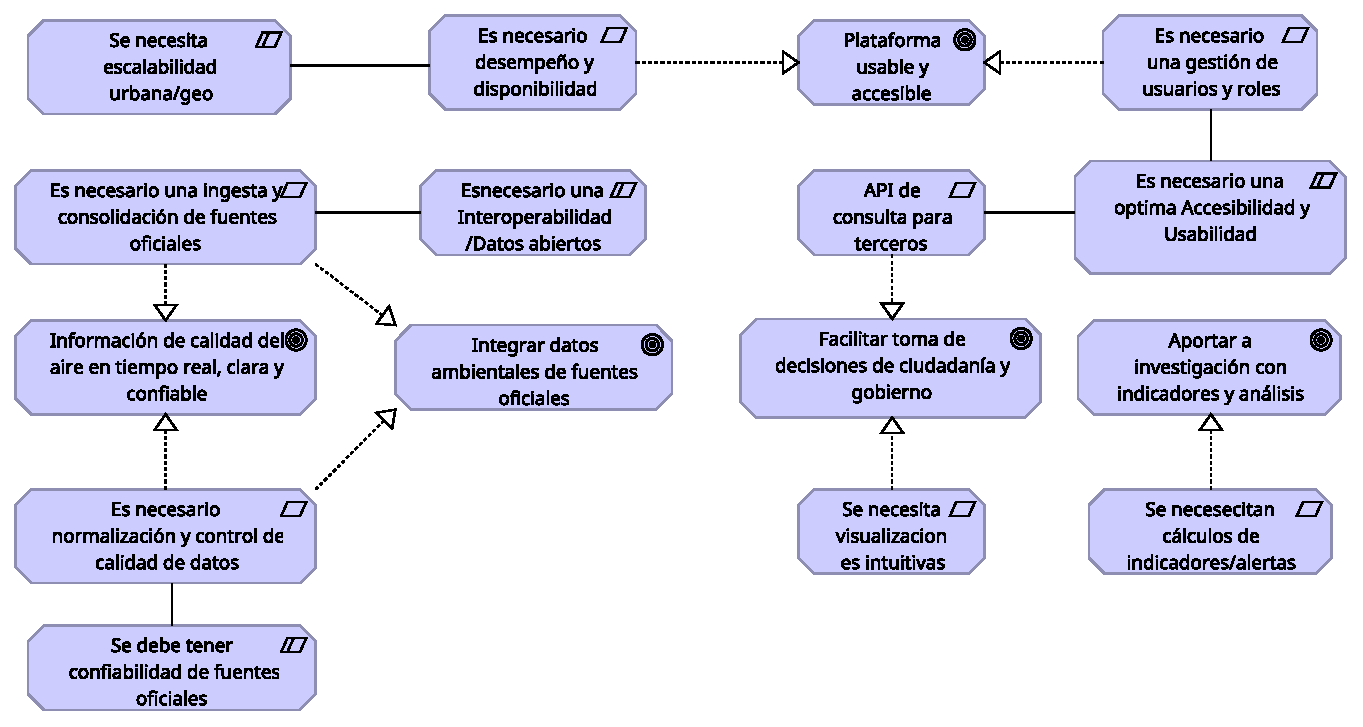
\includegraphics[scale=0.415]{\RCR/motivacion/Realizacion_Objetivos.pdf}
		\end{Marco}
	\end{NuevoParrafo}
	
	
	\begin{NuevoParrafo}{47}{20}[20][15]
		\begin{Marco}[\LineaSupC][\LineaInfC][\LineaIzqC][\LineaDerC][CBlanco]
			\subseccionC{\PVCOb}%{CTSeccionPrimeraPlana}{CCSeccionPrimeraPlana} 
			\centering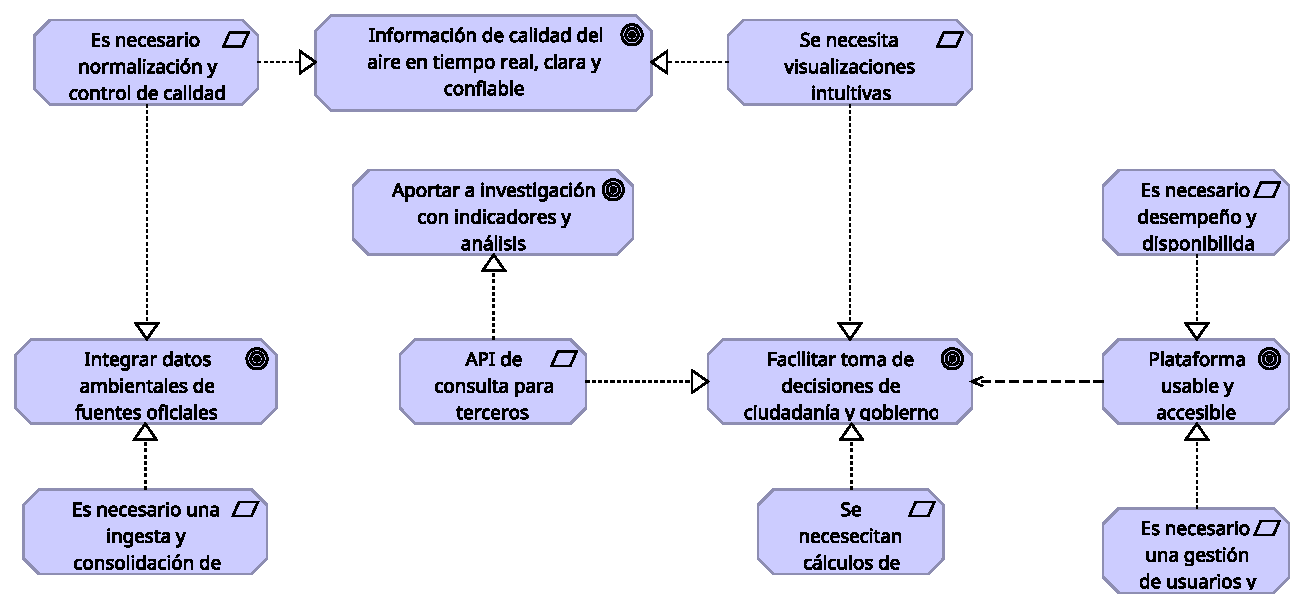
\includegraphics[scale=0.45]{\RCR/motivacion/Contribucion_Objetivos.pdf}
		\end{Marco}
	\end{NuevoParrafo}
	
	
	\begin{NuevoParrafo}{45}{41}[26][17]
		\begin{Marco}[\LineaSupC][\LineaInfC][\LineaIzqC][\LineaDerC][CBlanco]
			\subseccionC{\PVReR}%{CTSeccionPrimeraPlana}{CCSeccionPrimeraPlana} 
			\centering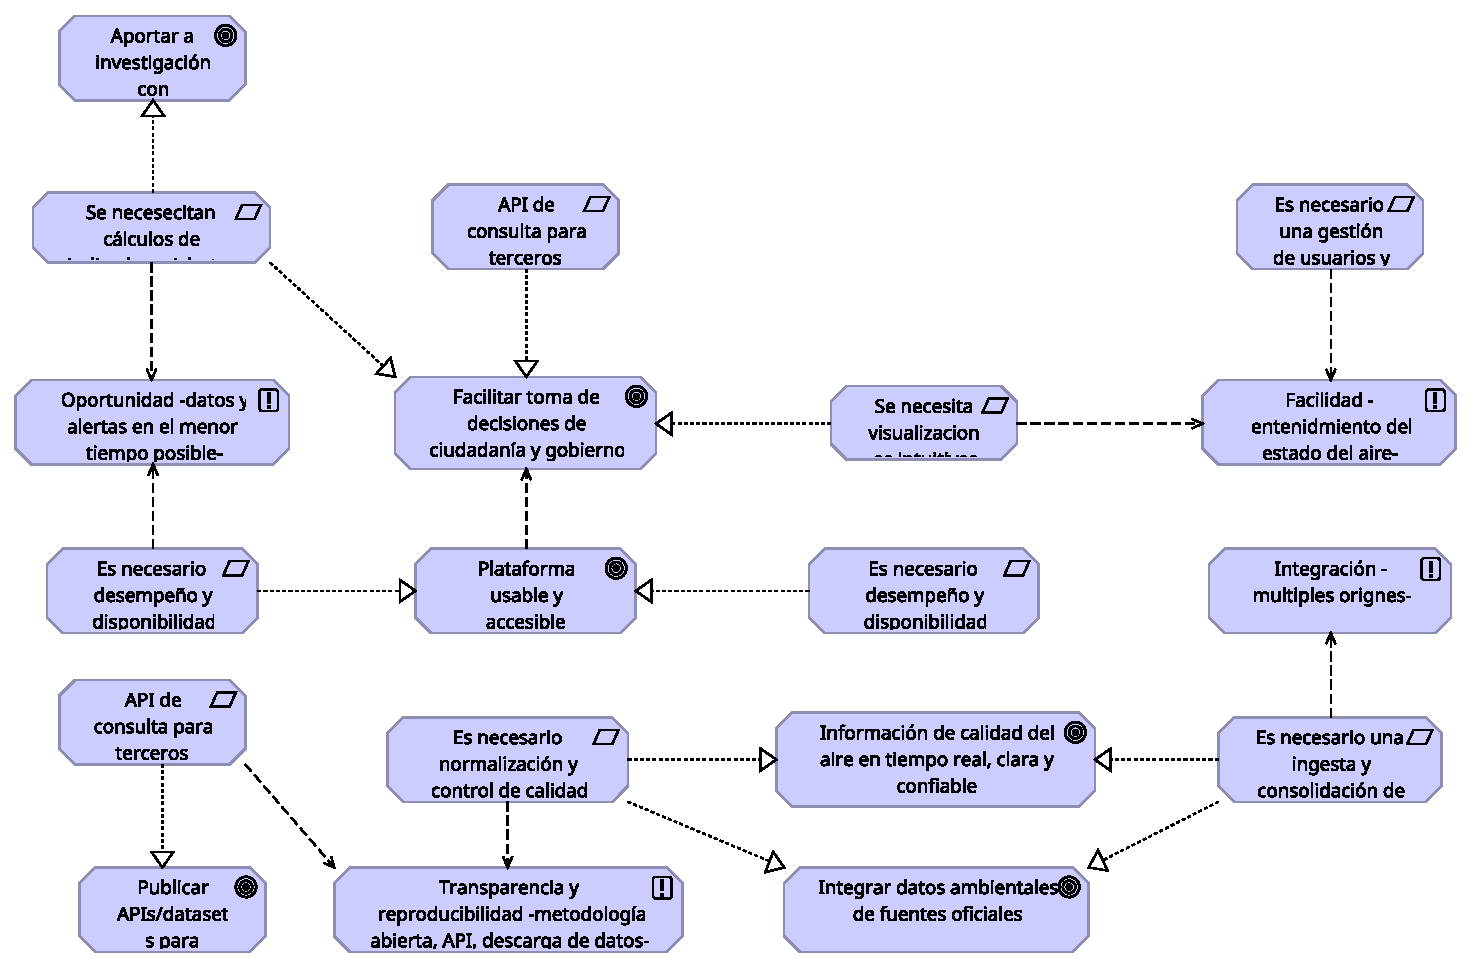
\includegraphics[scale=0.48]{\RCR/motivacion/Realizacion_Requerimientos.pdf}
		\end{Marco}
	\end{NuevoParrafo}
	\begin{NuevoParrafo}{45}{68}[26][17]
		\begin{Marco}[\LineaSupC][\LineaInfC][\LineaIzqC][\LineaDerC][CBlanco]
			\subseccionC{\PVMot}%{CTSeccionPrimeraPlana}{CCSeccionPrimeraPlana} 
			\centering\includegraphics[scale=0.5]{\RCR/motivacion/Motivacion.pdf}
		\end{Marco}
	\end{NuevoParrafo}

	%-----------------------------ORIGINAL---------------------------------------------
	% \begin{NuevoParrafo}{26}{0}[40][20]
	% 	\begin{Marco}[\LineaSupC][\LineaInfC][\LineaIzqC][\LineaDerC][CBlanco]
	% 		\subseccionC{MetaModelo}%{CTSeccionPrimeraPlana}{CCSeccionPrimeraPlana} 
	% 		\centering\includegraphics[scale=0.68]{\RMe MetaMotivacion.pdf}
	% 	\end{Marco}
	% \end{NuevoParrafo}
	
	% \begin{NuevoParrafo}{26}{41}[26][15]
	% 	\begin{Marco}[\LineaSupC][\LineaInfC][\LineaIzqC][\LineaDerC][CBlanco]
	% 	\subseccionC{\PVSta}%{CTSeccionPrimeraPlana}{CCSeccionPrimeraPlana} 
	% 	\centering\includegraphics[scale=0.68]{\RC/motivacion/Interesado.pdf}
	% 	\end{Marco}
	% \end{NuevoParrafo}
	
	% \begin{NuevoParrafo}{26}{68}[26][15]
	% 	\begin{Marco}[\LineaSupC][\LineaInfC][\LineaIzqC][\LineaDerC][CBlanco]
	% 		\subseccionC{\PVPri}%{CTSeccionPrimeraPlana}{CCSeccionPrimeraPlana} 
	% 		\centering\includegraphics[scale=0.68]{\RC/motivacion/Principios.pdf}
	% 	\end{Marco}
	% \end{NuevoParrafo}
	
	% \begin{NuevoParrafo}{47}{0}[20][15]
	% 	\begin{Marco}[\LineaSupC][\LineaInfC][\LineaIzqC][\LineaDerC][CBlanco]
	% 		\subseccionC{\PVROb}%{CTSeccionPrimeraPlana}{CCSeccionPrimeraPlana} 
	% 		\centering\includegraphics[scale=0.64]{\RC/motivacion/RealObjetivos.pdf}
	% 	\end{Marco}
	% \end{NuevoParrafo}
	
	
	% \begin{NuevoParrafo}{47}{20}[20][15]
	% 	\begin{Marco}[\LineaSupC][\LineaInfC][\LineaIzqC][\LineaDerC][CBlanco]
	% 		\subseccionC{\PVCOb}%{CTSeccionPrimeraPlana}{CCSeccionPrimeraPlana} 
	% 		\centering\includegraphics[scale=0.68]{\RC/motivacion/ContObjetivos.pdf}
	% 	\end{Marco}
	% \end{NuevoParrafo}
	
	
	% \begin{NuevoParrafo}{45}{41}[26][17]
	% 	\begin{Marco}[\LineaSupC][\LineaInfC][\LineaIzqC][\LineaDerC][CBlanco]
	% 		\subseccionC{\PVReR}%{CTSeccionPrimeraPlana}{CCSeccionPrimeraPlana} 
	% 		\centering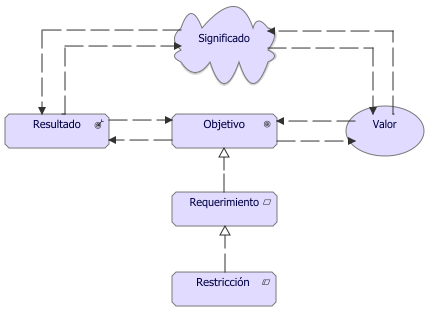
\includegraphics[scale=0.68]{\RC/motivacion/RealRequerimientos.pdf}
	% 	\end{Marco}
	% \end{NuevoParrafo}
	% \begin{NuevoParrafo}{45}{68}[26][17]
	% 	\begin{Marco}[\LineaSupC][\LineaInfC][\LineaIzqC][\LineaDerC][CBlanco]
	% 		\subseccionC{\PVMot}%{CTSeccionPrimeraPlana}{CCSeccionPrimeraPlana} 
	% 		\centering\includegraphics[scale=0.68]{\RC/motivacion/Motivacion.pdf}
	% 	\end{Marco}
	% \end{NuevoParrafo}

%%%%%%%%%%%%%%%%%%%%%%%%%%%%%%%%%%%%%%%%%%%%%%%%%%%%%%%%%%%%%%%%%%%%%%%%%%%%%%%%%%%%%%
\end{NuevaPagina}